\subsection{Attitude Determination and Control System (ADCS)}

The purpose of the ADCS (Attitude Determination and Control System) is to control
the orientation of a satellite with respect to an inertial frame of reference or
another entity such as stars, planets, other celestial bodies and certain fields.
An attitude system comprises of several components including, sensors, actuators,
algorithms and software**. An ADCS can come in the form of both passive and active
systems depending on the nature of the mission and the subsequent requirements of
each operational mode. Within this section the design process used for this
spacecraft mission is explained.

\subsubsection{Design process}
A design process is essential to facilitate the effective and optimised selection
of the hardware and software required to create the ADCS subsystem. The design
process utilised for this project can be seen in figure \ref{fig:adcs_design}.
The iterative loop placed within the Figure is symbolic of the mindset that was
taken throughout this system’s design, with the understanding of the various
requirements and constraints changing throughout the process with information
feeding in from the design of other subsystems.

\begin{figure}[h]
	\centering
	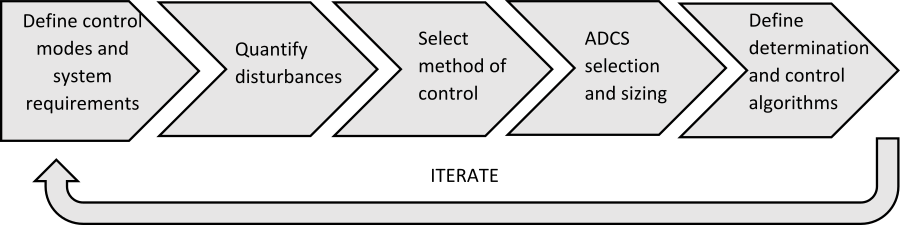
\includegraphics[width=\textwidth]{img/ADCS_design.png}
	\caption{Design process of the spacecraft ACDS}
	\label{fig:adcs_design}
\end{figure}

\subsubsection{Subsystem requirements}

When establishing the control modes and system requirements at the initial stage,
it was to consider what was needed to fulfill the mission objectives. Therefore,
some of the inputs into this design stage were the; mission requirements, mission
profile and mission constraints (cost, size and weight) etc. From this an initial
set of functional and performance requirements were set detailing the required
accuracy, reliability, rate of slew and others, useful in the later method of
control step.

\subsubsection{Control modes}

\paragraph{Detumble mode}

This mode is essential directly after the initial deployment of the satellite
constellation from the launch vehicle so stabilise the rotation of the satellites.
This mode also serves the purpose of a safe operating mode during the operational
life of the satellite, in the case of substantial disturbance torques, so that
the satellite’s rotation may be re-stabilised. It is preferable for de-tumbling
to occur as quickly as possible, so that the satellite can be reach a useful state.

Within this mode the satellite’s primary antenna must be directed over the earth’s
surface to enable data transmission and receipt with ground stations and devices.
This mode will also allow inter satellite communications between other satellites
due to the positioning of the secondary antenna’s. Within this stage the ADCS
requirements in terms of orientating the satellite are reduced, with only 2 axis
controls required to ensure the satellite antenna points directly to earth.

\paragraph{Thruster pointing mode}

This mode is needed during the early stages of the mission, post deployment,
whereby the satellites are to be positioned equidistant along their shared orbital
planes. It is preferable for thruster pointing to be as accurate as possible, so
as to minimise the required $\Delta V$ and thereby maximising fuel efficiency. This mode
may also be employed later in the life of the satellite, if fuel reserves remain.

\subsubsection{Disturbances}

The disturbance environment in which the spacecraft will operate helps to determine
which types of control methods will be required. For LEO spacecraft, such as the
satellite being designed within this project, there are four key types of
disturbance torques that need to be considered; gravity-gradient effects,
magnetic field torques, solar radiation pressures and aerodynamic torques.
The magnitudes of these disturbances depend on a variety of parameters including
orbital altitude and plane inclination. Within this mission for example,
the nature of the 8 different polar orbital planes employed for the constellation
will mean that some of the cubesats will receive more sun radiation compared than
others which in turn means a variation in solar radiation pressure disturbances
throughout the constellation.

The mass distribution and shape of the cubesat are important in determining the
centre of mass and the centre of pressure respectively. It’s ideal that for
all orientations of the spacecraft relative to aerodynamic and sun radiation
pressure disturbances, that the centre of pressure is as close to the centre
of mass to minimise the resultant disturbance moments. With the orbital height
known (625 km), some early approximations and assumptions for these disturbances
can be modeled and the values generated can be used in ADCS control method
selection. Disturbances from gravity-gradient effects will be less prevalent
throughout the life of these nanosatellites, due to their small size and symmetry
when pointed directly the earth, the ‘adjusted’ centre of gravity will be in line
with the satellites centre of mass.

Atmospheric drag:
\begin{equation}
	T_a = \frac{1}{2} \rho C_d A_r V^2 (cp_a - cm)
\end{equation}
, with $\rho$ the air density at orbital altitude, $C_d$ the drag coefficient,
$A_r$ the effective cross section, V the orbital speed, and $cp$, $cm$, the centers
of pressures and mass, respectively.

Magnetic torque:
\begin{equation}
	T_m = DB ~~~ D = \left(\frac{M}{R^3} \lambda \right)
\end{equation}

Gravity gradient:
\begin{equation}
	T_g = \frac{3\mu}{2R^3}\left|I_z - I_y\right| \sin2\theta
\end{equation}


Sun radiation pressure:
\begin{equation}
	T_s = \frac{\phi}{c} A_s (1+q) (cp_s - cm) \sin 2\phi
\end{equation}
